% третья часть

\section{Система учета потребления ресурсов}
Система учета ресурсов предназначена для считывания, мониторинга и работы с данными домовых счетчиков учета ресурсов. Данные со счетчиков попадают на сервер баз данных, в программе диспетчера и администратора данные отображаются, считаются, формируются отчеты. \cite{NK}

Проблемы:  
\begin{itemize}
	\item Некорректные начисления по оплате; 
	\item Неверная работа квартирных приборов учета (неисправности, воровство); 
	\item поставка ресурсов ненадлежащего качества (недогрев, перегрев, некачественная электроэнергия);
	\item Некорректная работа регулирующего теплового оборудования; 
	\item Отсутствие технической возможности проводного соединения с квартирными приборами учета.
\end{itemize}

Решение: 
\begin{enumerate}
	\item Создание единой облачной базы данных; 
	\item Конвертирование архивов ПУ различных производителей;
	\item Автоматизированный анализ данных.
\end{enumerate}

Система учета ресурсов состоит из:
\begin{itemize}
	\item Сервера баз данных;
	\item Контроллеры приборов учёта;
	\item Преобразователей интерфейса;
	\item Домовой сервер (Raspberry Pi);
	\item Службы сбора данных;
	\item Управляющей программы(администратора и диспетчера).
\end{itemize}
Администратор системы должен контролировать состояния на панеле мониторинга, добавлять новые счетчики, составлять отчеты, проводить аналитику. 

\subsection{Формирование единой базы данных}

\begin{enumerate}
	\item Опросом показаний занимается программа, запущенная на домовом сервере (Raspberry Pi).  Она должна извлекать данные о требуемых к опросу счетчиках из текстового файла (приложение 1.1), производить опрос и сохранять показания в отдельный текстовый файл (приложение 1.2). Опрос показаний должен производится 1 раз  в час (например в 05 минут каждого часа).
	\item Служба сбора данных производит непосредственный опрос всех Raspberry Pi. Эта программа устанавливается на сервер баз данных и производит выгрузку файлов data.txt  с домовых серверов в единую базу данных (FireBird, PostgreSQL) (приложение 2). После занесения данных в основную базу необходимо очистить файл data.txt.  Если в основной базе изменилась информация о счетчиках (порт, адрес КПУ или номер клеммы) данная программа должна загрузить новый файл counter.txt.
	\item Раз в сутки необходимо синхронизировать время домового сервера и сервера БД (это может быть отдельная программа или одна из функций программы из п.2).	
\end{enumerate}

\textbf{Квартирный учет ресурсов}

В квартирном учете применена проводная система снятия показаний. Для снятия показаний приборов учета с импульсным выходом применяется универсальный счетчик СКАУТ-КПУ, поддерживающий 12 импульсных входов. Приборы с протоколами передачи данных RS485, ModBUS и другими подключаются к плате сопряжения протоколов СКАУТ.

\textbf{Домовой учет ресурсов}

Домовые приборы учета с импульсным выходом применяются в комплекте со счетчиком импульсов СКАУТ-КПУ. При наличии у приборов внутреннего архива, опрос приборов и промежуточное хранение файлов архива осуществляется микрокомпьютером СКАУТ-Базовый

\subsection{монтаж: установка оборудования}

\begin{enumerate}
	\item Установить комплекс СКАУТ базовый в защитный шкаф
	\item Установить контроллер приборов учета
	\item Установить "умные" счетчики, с системой телеметрии на каждый вид ресурсов (газ, электроэнергия, вода, тепло)
	\item Проложить коммутационные кабели и подключить оборудование к сети связи
	\item Установить программное обеспечение на компьютер сотрудника УК
	\item Создать базы данных по счетчикам и адресам; провести пуско-наладочные работы
	\item Провести инструктаж сотрудников УК по использованию системы учета ресурсов
\end{enumerate}


\subsection{Автоматизированный анализ данных}

Коммунальные компании постоянно сталкиваются с неучтенными расходами воды.
Чтобы справиться с утечками и сократить неучтенные расходы воды, необходимо четко представлять себе ситуацию в распределительной сети. \cite{smartcity}

Наличие нужных данных в нужное время значительно облегчает борьбу с потерей и неучтенными расходами воды и повышает эффективность этих действий. Автоматизированная система учета отображает реальное состояние распределительной сети, помогает выявить различные типы неучтенных расходов и сократить потери воды. 

Рассмотрим проблему, когда от счетчика не поступает импульс. Есть два варианта:
\begin{itemize}
	\item Проблемы с самим счетчиком, например зависает счетный механизм
	\item Проблемы с телеметрией, обрыв линии, короткое замыкание, не исправен геркон
\end{itemize}

Ошибка №1. Проблемы со счетчиком ХВС. 

Потребление ХВС = 0 за сутки, при этом потребление ГВС > 0 за сутки.

Алгоритм поиска:

Находим разность между показаниями счетчиков ХВС и ГВС, за текущее число и за вчерашнее.
Оставляем значения счетчиков ХВС и ГВС, где разность ХВС = 0.
Убираем значения счетчиков ХВС и ГВС, где разность ГВС = 0.

Оставшиеся счетчики ХВС являются проблемными (можно сравнивать не за сутки, а за 3 или 5).

Ошибка №2. Проблемы со счетчиком ГВС.

Потребление ГВС = 0 за неделю, при этом потребление ХВС > 0 за неделю.

Алгоритм поиска:

Находим разность между показаниями счетчиков ХВС и ГВС неделю назад и за текущее число.
Оставляем значения счетчиков ХВС и ГВС, где разность ГВС = 0.
Убираем значения счетчиков ХВС и ГВС, где разность ХВС = 0.

Получили счетчики, которые попадают в поле подозрения.
Нужно провести отбор, возможно горячей водой просто не пользуются.

Убираем счетчики, у которых значения ГВС < 5 и значение ХВС < 10.
Оставшиеся счетчики ГВС являются проблемными и требуют ручной проверки.

Ошибка №3. Проблемы со счетчиком ХВС и ГВС.

Потребление ХВС = 0, ГВС = 0 за неделю, при этом потребление Э  >= Ср.Ар. за предыдущую неделю.

Алгоритм поиска:

Находим разность между показаниями счетчиков ХВС и ГВС неделю назад и за текущее число.
Оставляем значения счетчиков ХВС и ГВС, где разность ГВС = 0 и ХВС = 0.
Находим среднее арифметическое потребление электричества за предыдущую неделю.
Если потребление электроэнергии за неделю больше чем среднее арифметическое значение, то счетчики попадают в список проблемных счетчиков.

Ошибка №4. Проблемы с электросчетчиком.

Потребление Электричества = 0 за сутки, при этом потребление ХВС > 0 и/или ГВС > 0 за сутки и более.

\subsection{Анализ показаний приборов учета}

Учет и анализ коммунальных ресурсов дает возможность выявить их перерасход, вызванный, возможно, и халатным отношением, либо неисправностью приборов учета. Также становится прозрачным перерасход ресурсов и несанкционированное их потребление.\cite{journal}

«Личный кабинет» программы СКАУТ позволяет получить часовые, суточные и ежемесячные данные в виде таблиц и графиков, что позволяет удобно анализировать расход ресурсов.

Детализация данных для всестороннего анализа.
Посуточная статистика. Пример приведен на рис.~\ref{fig:day}
\begin{figure}[H]
	\centering
	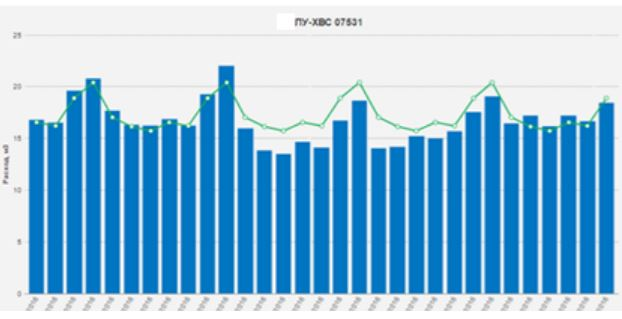
\includegraphics[width=0.7\linewidth]{pics/day}
	\caption{Посуточное потребление}
	\label{fig:day} 
\end{figure}
Почасовая статистика. Пример приведен на рис.~\ref{fig:hour}
\begin{figure}[H]
	\centering
	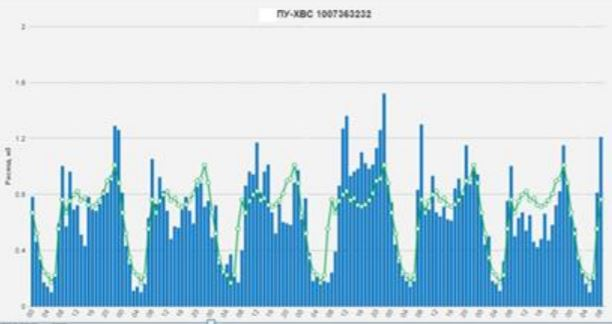
\includegraphics[width=0.7\linewidth]{pics/hour}
	\caption{Почасовые показания}
	\label{fig:hour} 
\end{figure}

С выведением информации по средне статическому потреблению.
Графическое представление, особенно за длительные сроки, даёт наглядную картину работы водосчетчиков и электросчетчиков. 

Несколько сложнее обнаруживать утечки в системе горячего водоснабжения. Непрерывный и неравномерный разбор горячей воды затрудняет их определение. Использование статистики потребления горячей воды жилым домом в ночные часы (3 часа ночи) позволяет улавливать фоновые потери для каждого дома. В основном это передавливание горячей воды в трубопровод холодного водоснабжения через неисправные квартирные смесители. Установив для каждого дома фоновый уровень потерь, можно контролировать появление протечек. До настоящего времени нами не было обнаружено таких протечек, однако данным методом в Обнинске были выявлены два 100 квартирных дома, где фоновое потребление холодной воды на дом достигало 600 литров в час и более. В квартирах одного их них были обнаружены два неисправных сливных бачка, в другом доме протекал вентиль в подвале, и вода уходила в ливневую канализацию. После ремонтов фоновое потребление в этих домах установилось на уровне 250–300 литров в час. \cite{journal2}

Так же известно, что потребление горячей воды не может превышать потребление холодной. Данная проблема сигнализирует нам об неисправности счетчика. С помощью наложения двух графиков потребления горячей и холодной воды, можем наглядно увидеть проблемные счетчики.